\chapter{An information-theoretic foundation for posterior agreement}
\chaptermark{Posterior agreement}

%\newcommand{\prob}{\mathbb{P}}
%\newtheorem{assumption}{Assumption}
\newtheorem{objective}{Objective}

%
%\newcommand{\carlos}[1]{}
%\newcommand{\fcarlos}[1]{}
%\newcommand{\todo}[1]{}
%
%\theoremstyle{definition}
%
%\newtheorem{definition}{Definition}
%\newtheorem{example}{Example}
%\newtheorem{theorem}{Theorem}

\section{Introduction}

This chapter proposes an information-theoretic foundation for posterior agreeement, as a method for validating clustering algorithms, originally proposed by Joachim Buhmann~\cite{buhmann2010information} and studied by Alex Gronskiy as part of his doctoral thesis~\cite{gronskiy2018statistical}.
 
Posterior agreement can be understood as a method for \emph{validating algorithms} that solve stochastic optimization problems of the form
%
$$\min_{c} \mathbb{E}_X\left[R(c, X)\right].$$
% 
Here, $R(c, X)$ is the result of evaluating a cost function on a candidate solution $c$ on an instance of the problem described by the random variable $X$. The expectation is computed with $X$'s distribution.

In posterior agreement, we assume that an algorithm is a function that computes, from a given observation $X'$, a \emph{posterior distribution} $p(\cdot \mid X')$ over a finite space $\mathcal{C}$ of possible solutions. Every algorithm can be converted into such an algorithm, even if it is deterministic. In this case, the posterior distribution is just a distribution that assigns probability mass one to the algorithm's output.

Posterior agreement assesses the performance of an algorithm by computing the \emph{expected log posterior agreement}:
%
\begin{equation}
\mathbb{E}_{X', X''} \log \left(\left|\mathcal{C}\right|\kappa\left(X', X''\right)\right),
\label{eq:overview_exp_log_post_agr}
\end{equation}
%
where $\kappa\left(X', X''\right)$ is the \emph{posterior agreement kernel}:
%
$$\kappa\left(X', X''\right) := \sum_{c \in \mathcal{C}} p(\cdot \mid X')p(\cdot \mid X'').$$

The expected log posterior agreement requires the joint probability distribution of $X'$ and $X''$, which is often unknown. One only has access to a handful of observations, at least two: $X'$ and $X''$. In this case, one can use the \emph{empirical log posterior agreement}:
%
\begin{equation}
\log \left(\left|\mathcal{C}\right|\kappa\left(X', X''\right)\right).
\label{eq:overview_emp_log_post_agr}
\end{equation}

Moreover, the empirical log posterior agreement is intended to be a metric to compare different algorithms. Therefore, it is often sufficient to measure $\kappa\left(X', X''\right).$

%We show how posterior agreement can compare, for example, Prim's, Kruskal's, and the reverse-delete algorithm for computing spanning trees for graphs whose edge weights are defined by random variables, as in the example above. Posterior agreement can also compare among different cost functions and hyperparameter values, when training machine learning models.

Therefore, posterior agreement advocates that, in the context of stochastic optimization, \emph{algorithms should aim for maximizing the posterior agreement kernel, given two instances of the problem}, rather than minimizing the cost function for either instance or an aggregate of these instances.

The proofs given in this chapter works for algorithms that satisfy the following \emph{asymptotic equipartition property}. As $n \to \infty$, $\log \left(\left|\mathcal{C}\right|\kappa(X', X'')\right)$ converges in probability to
%
\begin{equation}
\mathbb{E}_{X', X''}\left[\log \left(\left|\mathcal{C}\right|\kappa(X', X'')\right)\right].
\end{equation}
%
Such property is satisfied by many of the algorithms studied in this script, like deterministic annealing and histogram clustering. Furthermore, if an algorithm produces distributions that can be sufficiently well approximated by a mean-field approximation, then it is possible to demonstrate that they also fulfil this asymptotic equipartition property.

\begin{exercise}
Show that deterministic annealing (DA) satisfies the asymptotic equipartition property.
\end{exercise}

\begin{proof}
Recall that the distribution $p(\cdot \mid \theta, X')$ computed by DA on a given sample of points $X' = \{x'_1, \ldots, x_n'\}$ factorizes as follows:
%
\begin{equation}
p(c \mid \theta, X') = \prod_{i \leq n} p(c(i) \mid \theta, x'_i),
\end{equation}
%
where
%
\begin{equation}
p(k \mid \theta, x'_i) \propto \exp\left(-\frac{1}{T}\left\|x_i - \theta_k\right\|^2\right).
\end{equation}
%
From Exercise~\ref{ex:pa_factorizes_da}, we know that
%
\begin{equation}
\kappa\left(X', X''\right) = \prod_{i \leq n} \sum_{k \leq K} p(k \mid \theta, x'_i)p(k \mid \theta, x''_i).
\end{equation}
%
Therefore,
%
\begin{equation}
\log \left(\left|\mathcal{C}\right|\kappa\left(X', X''\right)\right) = \log \left|\mathcal{C}\right| + \sum_{i \leq n}\log \sum_{k \leq K} p(k \mid \theta, x'_i)p(k \mid \theta, x''_i).
\end{equation}
%
Now, if we take the limit as $n \to \infty$ of both sides, and apply the law of large numbers, we have that, as $n \to \infty$, $\log \left(\left|\mathcal{C}\right|\kappa\left(X', X''\right)\right)$ converges in probability to
%
\begin{equation}
\log \left|\mathcal{C}\right| + n \mathbb{E}_{x', x''}\left[\log \sum_{k \leq K} p(k \mid \theta, x')p(k \mid \theta, x'')\right],
\label{eq:result_conv_prob_pa}
\end{equation}
%
Finally, observe that
%
\begin{align}
\mathbb{E}_{X', X''}\left[\log \kappa\left(X', X''\right)\right]
&= \mathbb{E}_{X', X''}\left[\sum_{i \leq n}\log \sum_{k \leq K} p(k \mid \theta, x'_i)p(k \mid \theta, x''_i)\right]\\
&= \sum_{i \leq n}\mathbb{E}_{X', X''}\left[\log \sum_{k \leq K} p(k \mid \theta, x'_i)p(k \mid \theta, x''_i)\right]\\
&= \sum_{i \leq n}\mathbb{E}_{x'_i, x''_i}\left[\log \sum_{k \leq K} p(k \mid \theta, x'_i)p(k \mid \theta, x''_i)\right]\\
&= n\mathbb{E}_{x', x''}\left[\log \sum_{k \leq K} p(k \mid \theta, x')p(k \mid \theta, x'')\right].\\
\end{align}
%
Substituting this in Equation~\ref{eq:result_conv_prob_pa} yields the desired result.
\end{proof}

\begin{corollary}
Consider an algorithm that, when given as input a sample $X'$, outputs a distribution $p(\cdot \mid X')$. Assume that this distribution admits a mean-field approximation such that
%
\begin{equation}
p(c \mid X') \approx \prod_{i \leq n} q(c_i \mid x_i').
\end{equation}
%
Then this algorithm fulfils the asymptotic equipartition property.
\end{corollary}

The proof is analogous to the one above.

%\todo{Organization of these notes.}

\section{Motivation}

\begin{figure}
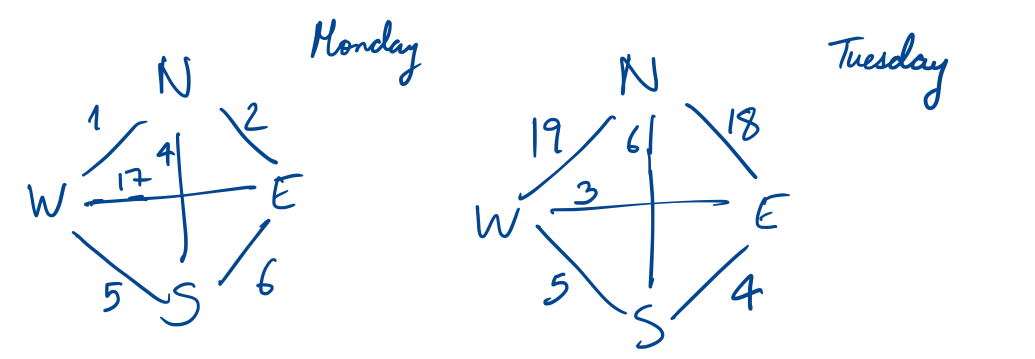
\includegraphics[width=\textwidth]{\dir/mst_setup.png}
\caption{A graph with its observed edge weights for two different days.}
\label{fig:mst_setup}
\end{figure}

Figure~\ref{fig:mst_setup} gives two graphs modeling a city with four main locations: North, East, South, and West. There is a road connecting any two different locations and, depending on the day, traversing that road by car takes some amount of time. The number labeling each edge indicates that time. Observe that the time varies with each day.

Consider the minimum spanning tree of each of these two graphs. For Monday's graph, the tree is the one with North at the root and all other locations as children of North. For Tuesday's graph, the tree is the one with South at the root and all other locations as children of South. We call these two trees the North and South trees, respectively.

Can we estimate from this information what Wednesday's graph's minimum spanning tree will look like?

The city graph can be understood as a random variable $X$. More precisely, it is a collection of 6 random variables, each of them defining an edge's weight on a particular day. Hence, the weight $R(c, X)$ of a tree $c$ in $X$, which is the sum of the edge weights in $c$, is also a random variable. We can then formulate the problem of the minimum spanning tree for our case as the following stochastic optimization problem:
%
\begin{equation}
\arg \min_{c \in \mathcal{C}} \mathbb{E}_X\left[R(c, X)\right],
\label{eq:stoch_min_span_tree}
\end{equation}
%
where $\mathcal{C}$ denotes all spanning trees of the city graph.

This type of optimization problems appear very often in combinatorial optimization and statistical learning. One challenge in this type of optimization problems is that we do not know $X$'s probability distribution.
One natural way to go around this issue and approximately solve Problem~\ref{eq:stoch_min_span_tree} is to substitute $\mathbb{E}\left[R(c, X)\right]$ with an \emph{empirical estimate}:
%
$$\mathbb{E}\left[R(c, X)\right] \approx \frac{1}{N}\sum_{i \leq N} R(c, X_i),$$
%
where $\left\{X_1, \ldots, X_n\right\}$ is a sample of observed values of $X$.

When $n$ is sufficiently large and each $X_i$ is independent from the others, then by the law of large numbers, this becomes a good approximation of $\mathbb{E}\left[R(c, X)\right]$. We call the \emph{empirical risk minimizer} the solution of the problem:
%
\begin{equation}
\arg \min_{c \in \mathcal{C}} \sum_{i \leq n}\left[R(c, X_i)\right],
\label{eq:erm}
\end{equation}

Unfortunately, the empirical risk minimizer does not always minimize the expected risk, especially, when the sample size $n$ is small, as we saw in the random array problem in Section~\ref{sec:random_array}. The empirical risk minimizer can overfit the sample and, therefore, fail to generalize to other samples.

One can prevent such overfitting with techniques like regularization. This makes the solutions less sensitive to the noise in the sample. However, such techniques may lead to solutions that are too insensitive to the signal in the sample, failing to minimize the expected cost as well.

Solving Problem~\ref{eq:stoch_min_span_tree} requires designing algorithms that strike a balance between two extremes. On one hand, algorithms may \emph{overfit} and produce solutions that are too sensitive to the noise in the sample. On the other hand, algorithms may \emph{underfit} and produce solutions that are too insensitive to the signal in the sample. 
%These two extremes are illustrated in Figure\ref{fig:clustering}\todo{} for the problem of clustering. 
These two extremes can be illustrated in the case of clustering.
In the overfitting extreme, an algorithm may just make each point in the sample its own cluster (and this solution would actually minimize the expected cost). In the undefitting extreme, an algorithm may just put all points in the sample into one single cluster. The overfitting algorithm minimizes the cost, but is extremely sensitive to noise in the data, whereas the underfitting algorithm is very robust, but fails to minimize the expected cost. Can we find a common ground between these two?

%We present later scenarios where the empirical risk minimizer is not the best solution we can obtain, especially when we have only very few observations. One example, presented in Section~\ref{sec:random_array} is the problem of computing the minimum of an array $X = \left(X_1, \ldots, X_n\right)$ of random variables. Given just two observations $X^1$ and $X^2$, estimating $\min_i \mathbb{E}_X[X_i]$ with the empirical risk minimizer is not the best we can do. We also showed in that section, how combining maximum entropy and posterior agreement yielded a better estimator.

\subsection*{Posterior agreement}

To find a solution to this apparent dilemma, posterior agreement has been proposed. This is a metric to evaluate how well an algorithm proposes solutions that minimize the expected cost and, at the same time, that are robust to the noise in the data.

Why is posterior agreement a good metric for validating algorithms? Why should we use it instead of other more standard criteria like cross-validation or the minimum description length? These notes argue that posterior agreement is effective, \emph{because it quantifies the amount of information that algorithms extract from phenomena}.
%Moreover, there are also scenarios where it is not possible to get a sufficiently large sample of observed values to estimate $X$'s distribution. \carlos{Give examples of such scenarios}

\section{Overview}
%
%For example, in the context of computing the city graph's minimum spanning tree, the phenomenon is the probability distribution that governs the edge weights that we observe on a particular day. An observation $X'$ defines the actual edge weights of a particular day. The signal we want to retrieve is a distribution $p(\cdot)$ over the spanning trees. For a spanning tree $c$, $p(c)$ measures how much we believe that minimizes $\mathbb{E}\left[R(c, X)\right]$.

Posterior agreement originates from formalizing an algorithm $\mathcal{A}$ \emph{as a communication channel} by which a sender and a receiver communicate outputs from $\mathcal{A}$. The main argument justifying posterior agreement states the following. The amount of information conveyed by an algorithm can be measured by the \emph{capacity} of that communication channel, where the capacity, as we explain later, defines the maximum number of distinguishable messages that can be communicated through the channel.

This section gives an informal overview of this main argument. The later sections formalize this argument. We start with a recap of Shannon's channel coding theory and then show how to apply it to represent and analyze algorithms as communication channels.

\subsubsection*{Shannon's channel coding theorem}

Consider a channel by which a sender can transmit bits to a receiver. Assume that the channel is noisy in the sense that a bit can be flipped during transmission with probability $\epsilon < 0.5$. The sender and the receiver agree on transmitting only bitstrings of length $n$. We call these bitstrings \emph{codewords}. 

Observe that if $\epsilon = 0$, then the sender can reliably communicate $2^n$ different messages to the receiver, by agreeing in advance with the receiver on a way to encode each message as one codeword of length $n$. This correspondence is called a \emph{code} and will be formally defined in Section~\ref{sec:shannon_theorem}.

In practice, $\epsilon > 0$. Therefore, the sender and the receiver need to agree on a code that is robust to the channel's noise. We now show two examples of codes:

\begin{itemize}
\item They could agree on just 2 messages, encoded as $00\ldots0$ and $11\ldots 1$, respectively. If the codeword length is sufficiently large, then with high probability, less than half of the bits will be flipped during transmission. As a result, the receiver can almost surely identify the message from the received codeword, by just counting the frequency of each bit in the codeword.
\item They agree on sending $2^n$ messages, each encoded with a unique codeword of length $n$. With high probability, some of the bits will be flipped during transmission and the receiver will fail to identify the message that the sender tried to communicate.
\end{itemize}

Observe that these two codes represent two extremes, as $n \to \infty$. On one hand, the first code is robust: it communicates only 2 messages, but with high probability of success. On the other hand, the second code communicates the maximum number of possible messages, but with low probability of success, as it is very sensitive to the channel's noise. One can also imagine other codes that strike a balance between the number of messages to be communicated and the success probability. Observe how these two extremes correspond to the two extremes of overfitting and underfitting. 

Shannon's coding theorem answers the following question. \emph{What is the code that maximizes the number of messages that the sender can communicate to the receiver, while attaining a probability of success close to 1, as $n \to \infty$?} When $\epsilon > 0$, this number is clearly below $2^n$, but since $\epsilon < 0.5$, this number must be positive. Shannon shows that this number is $2^{nc}$, where $c$ is \emph{the channel's capacity}, a quantity that is defined by the channel. Therefore, channels with higher capacity allow the communication of more messages at the same codeword length.

\subsubsection*{Posterior agreement}

Posterior agreement originates by adapting Shannon's coding theorem to the context of algorithms. This requires a way of modeling an algorithm $\mathcal{A}$ as a communication channel $C_{\mathcal{A}}$, where a sender communicates outputs from $\mathcal{A}$ to a receiver. We do this in these notes and argue that the capacity of $C_{\mathcal{A}}$ is defined by $\mathcal{A}$'s ability to compute robust solutions that minimize the expected cost. That is, if $\mathcal{A}$ is a robust minimizer of the expected cost, then it is possible to communicate many more messages through $C_{\mathcal{A}}$ than when $\mathcal{A}$ is sensitive to noise or when $\mathcal{A}$ is a poor minimizer of the expected cost.

We give an informal overview of this argument next. A rigorous argument is given in Section~\ref{sec:comm_protocol}.

We assume given an \emph{instance space} $\mathcal{X}$, comprising all possible observations, and a \emph{solution space} $\mathcal{C}$, comprising all possible solutions. A phenomenon is then a probability distribution over $\mathcal{X}$. We assume that algorithms intending to solve Problem~\ref{eq:stoch_min_span_tree} receive in the input an observation $X'$ and output a distribution $p(\cdot \mid X')$ over $\mathcal{C}$.

For our analysis, we assume that each instance space contains all observations of a given ``size'' $n \in \mathbb{N}$. This size $n$ is a notion that measures the observations' and phenomena's complexity. For example, in the minimum spanning tree problem, an instance space contains only all weighted graphs with a fixed number $n$ of vertices.

For an algorithm $\mathcal{A}$, we define a communication channel $C_{\mathcal{A}}$ that works as follows. To use the channel, a sender picks an instance $X'$, drawn from a phenomenon $p_X$, computes and inputs $p(\cdot \mid X')$ to the channel. The channel replaces $p(\cdot \mid X')$ with $p(\cdot \mid X'')$, where $X''$ is a fresh new instance drawn from $p_X$. The channel outputs $p(\cdot \mid X'')$ to the receiver.

We now emphasize the key insight of this modeling. If $\mathcal{A}$ is robust to the fluctuations in $X'$, then there should not be much difference between $p(\cdot \mid X')$ and $p(\cdot \mid X'')$. In contrast, if $\mathcal{A}$ is very sensitive to the fluctuations in $X'$, then $p(\cdot \mid X')$ and $p(\cdot \mid X'')$ may be very different. Hence, $\mathcal{A}$'s robustness to noise defines how many different ``messages'' can we send through this channel. We conclude then that $\mathcal{A}$'s robustness is measured by the capacity of this channel $C_{\mathcal{A}}$. This capacity, as we show in Section~\ref{sec:comm_protocol}, can be estimated by the expected log posterior agreement. For this reason, we argue that algorithms intended to solve Problem~\ref{eq:stoch_min_span_tree} shall be measured by their expected log posterior agreement.

%Observe the following analogies to Shannon's coding theory. Channels have a capacity that define the maximum number of distinguishable messages that can be communicated. Channels with higher capacity are preferable, as they allow more different messages to be communicated. Analogously, we argue that algorithms can be modeled as channels and, therefore, have a capacity, which we later show to be the expected log posterior agreement. Hence, we argue that algorithms with higher expected log posterior agreement are preferable, as they allow more different messages to be communicated.

\subsubsection*{Protocol overview}

We now introduce a protocol describing a code by which a sender can communicate messages to a receiver. Let $\mathcal{A}$ be an algorithm intending to solve Problem~\ref{eq:stoch_min_span_tree}. In our case, a message is a phenomenon and a codeword is the output $p(\cdot \mid X')$ of $\mathcal{A}$ when given an observation $X'$ from a phenomenon as input. 
%Analogous to Shannon's coding theorem, the sender and the receiver aim to maximize the number of different messages that the sender can communicate, while ensuring that the receiver's probability of success goes to 1 as $n \to \infty$.

Figure~\ref{fig:overview_protocol} illustrates the idea behind the protocol. The sender must describe a phenomenon $q$ to a receiver through a noisy channel. The sender makes an observation $X'$ from $q$, uses $\mathcal{A}$ to compute $p(\cdot \mid X')$, and sends through the channel to the receiver. The channel is noisy and we represent its noise by replacing $p(\cdot \mid X')$ with $p(\cdot \mid X'')$, where $X''$ is another observation from $q$. The receiver succeeds if he is able, using $p(\cdot \mid X'')$, to identify $q$. Observe how this protocol measures the informativeness of an algorithm by the ability of the receiver to identify phenomena, given the algorithm's output.

\begin{figure}
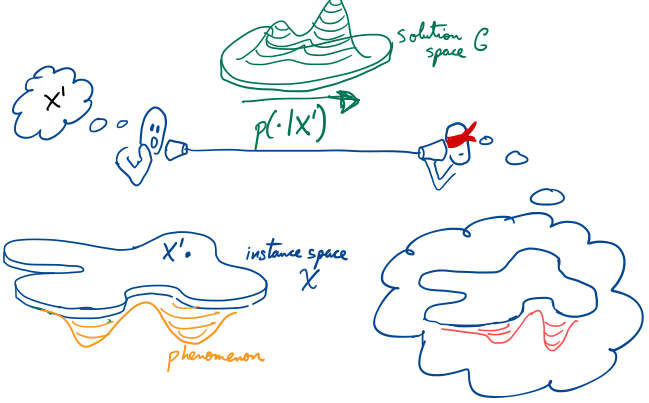
\includegraphics[width=\textwidth]{\dir/overview_protocol.png}
\caption{}
\label{fig:overview_protocol}
\end{figure}

We remark that this protocol is just a thought experiment. The protocol is computationally impossible for many interesting optimization problems. This is because the protocol requires that we know the underlying distribution behind the observations of one phenomenon. This is not possible in most of the cases. Nonetheless, the protocol provides a formal justification and motivation for posterior agreement.

\subsubsection*{Protocol example}

We now give a more precise overview by showing how posterior agreement works with a simple example. Let $\mathcal{A}_1$ and $\mathcal{A}_2$ be two algorithms that estimate the mean of a univariate distribution, given only a sample from that distribution. For example, $\mathcal{A}_1$ fits a Gaussian to the sample via maximum-likelihood estimation whereas $\mathcal{A}_2$ does the same, but only using only the maximum and the minimum of that sample. Suppose that both algorithms output Gaussian distributions that indicate where they believe that the mean is. 

The protocol works as follows. Fix $n \in \mathbb{N}$, which denote the size of all the observations in the instance space. In our case, $n$ denotes the sample size. The sender and the receiver are given the algorithm under evaluation $\mathcal{A}_i$ and then they choose the size $m_n \in \mathbb{N}$ of the set of messages that the sender will attempt to communicate. Recall that they want to choose $m_n$ as large as possible. However, a large $m_n$ increases the probability $P_n$ that the receiver fails to recognize the message from the codeword transmitted by the sender. We later see that the best choice for $m_n$ is defined by $\mathcal{A}_i$. 

The protocol proceeds then as follows:

\begin{enumerate}
\item\label{step:sample_observations} (Figure~\ref{fig:agree_on_code}) The sender and the receiver agree on a set of $m := m_n$ phenomena, which we represent with the probability distributions $q_1, q_2, \ldots, q_m$.
\item (Figure~\ref{fig:agree_on_code}) The sender and the receiver together make one observation $X'_i$ of each phenomenon $q_i$, with $i \leq m$. In this case, an observation is a sample of points from $q_i$. Afterwards, they use $\mathcal{A}_j$, with $j \in \{1, 2\}$, to compute a distribution $p(\cdot \mid X')$ for each observation $X'$.
\item\label{step:choose} (Figure~\ref{fig:noisy_channel}) An observation $X'$ is chosen out of these $m$ observations uniformly at random. $X'$ is given to the sender, but kept secret from the receiver.
\item (Figure~\ref{fig:substitution_maneuver}) The sender sends $p(\cdot \mid X')$ to the receiver through the communication channel $C_{\mathcal{A}_j}$, defined by $\mathcal{A}_j$. This channel replaces $p(\cdot \mid X')$ with $p(\cdot \mid X'')$, where $X''$ is a fresh new observation from the same phenomenon where $X'$ comes from.
\item (Figure~\ref{fig:guessing}) The receiver gets $p(\cdot \mid X'')$ and must now guess which observation in $\{X'_1, \ldots, X'_m\}$ the sender chose in Step~\ref{step:choose}. For this, the receiver uses the natural approach of guessing the observation $\hat{X}$ for which $p(\cdot \mid \hat{X})$ overlaps the most with $p(\cdot \mid X'')$. In other words, the receiver guesses the observation $\hat{X}$ that fulfills:
%
$$\kappa\left(\hat{X}, X'\right) \geq \kappa\left(Y, X'\right), \text{ for all Y.}$$
%
\item If $\hat{X} = X'$, the receiver has succeeded.
\end{enumerate}

\begin{figure}
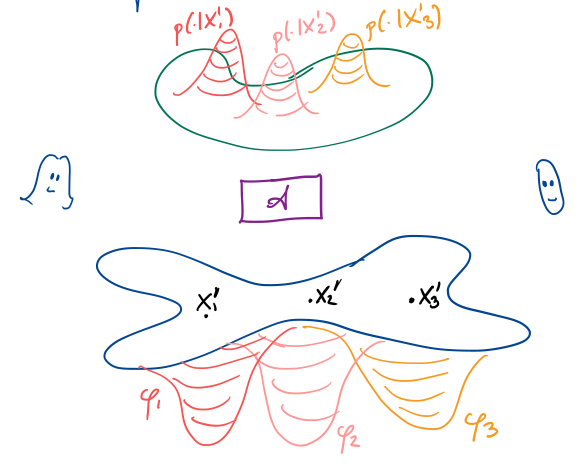
\includegraphics[width=\textwidth]{\dir/agree_on_code.png}
\caption{}
\label{fig:agree_on_code}
\end{figure}

\begin{figure}
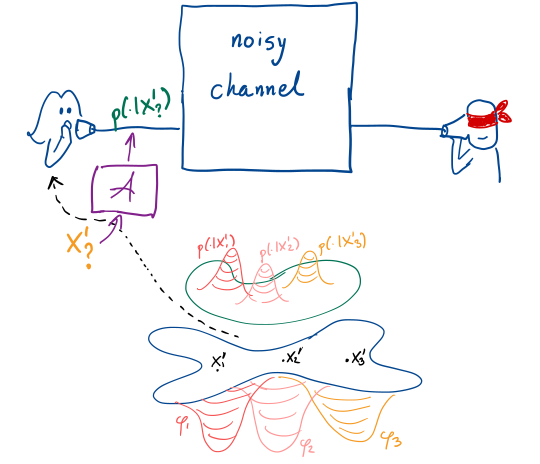
\includegraphics[width=\textwidth]{\dir/noisy_channel.png}
\caption{}
\label{fig:noisy_channel}
\end{figure}

\begin{figure}
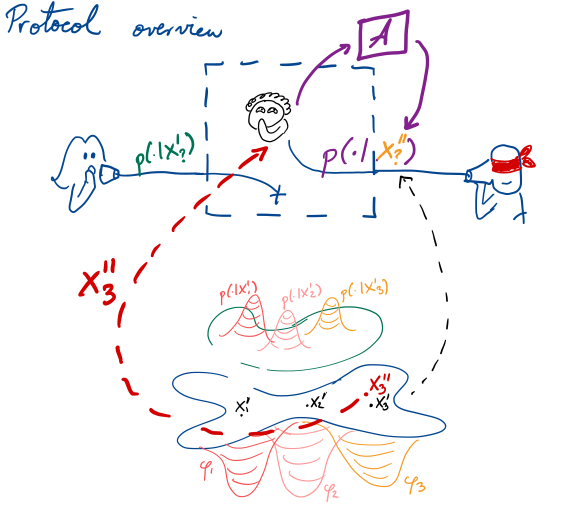
\includegraphics[width=\textwidth]{\dir/substitution_maneuver.png}
\caption{}
\label{fig:substitution_maneuver}
\end{figure}

\begin{figure}
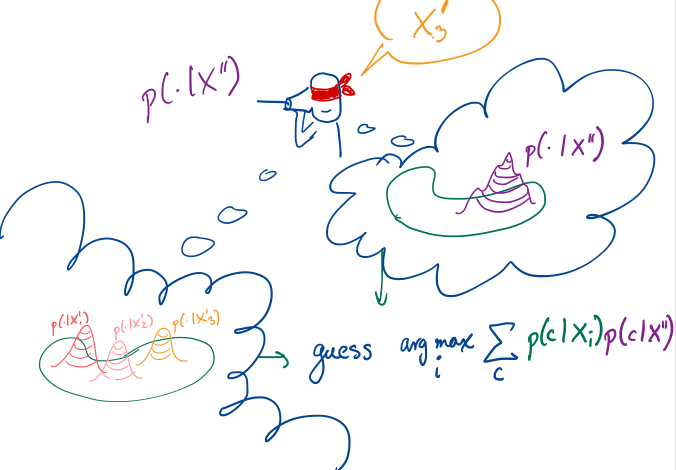
\includegraphics[width=\textwidth]
{\dir/guessing.png}
\caption{}
\label{fig:guessing}
\end{figure}

\subsubsection*{Receiver's probability of failure}

We show in Section~\ref{sub:prob_comm_error} that the receiver's failure probability is bounded above by 
%
$$\exp\left(- \mathbb{E}_{X', X''} \left[\log \left(\left|\mathcal{C}\right|\kappa\left(X', X''\right)\right)\right] + \epsilon \log \left|\mathcal{C}\right| + \log m\right),$$ 
%
where $\epsilon > 0$ is arbitrary, $\mathcal{C}$ is the solution space, and $m$ is the number of observations defined in Step~\ref{step:sample_observations}.

Assume now that $\log \left|\mathcal{C}\right| = \Omega(n)$. This is a reasonable assumption, as for many interesting problems, $\mathcal{C}$ grows exponentially in $n$. Observe that the algorithm can only influence $\kappa\left(X', X''\right)$. If $\epsilon$ is sufficiently small and the algorithm ensures that 
%
$$\mathbb{E}_{X', X''} \log\left(\left|\mathcal{C}\right| \kappa\left(X', X''\right)\right) - \log m = \Omega(n),$$ 
%
then the receiver's failure probability becomes $0$ as $n \to \infty$. The algorithm can ensure this by \emph{maximizing the expected log posterior agreement}. The larger this quantity is, the higher $m$ can be and the more messages the sender can communicate to the receiver.
%
%\begin{figure}
%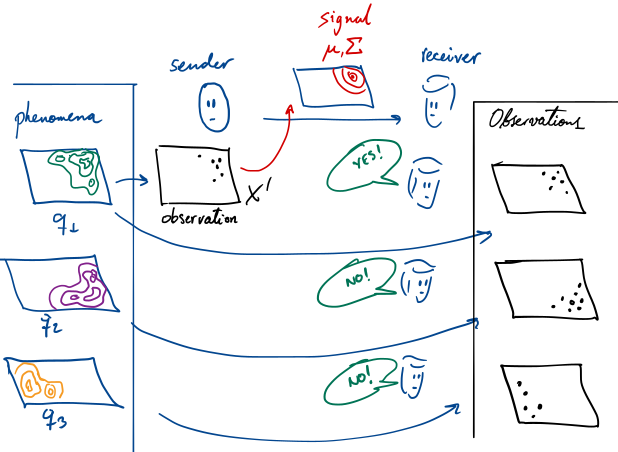
\includegraphics[width=\textwidth]{stoch_opti_as_comm.png}
%\caption{Stochastic optimization as a communication. The sender makes an observation $X'$ of a phenomenon $q_1$. The sender computes a signal $p(\cdot \mid X')$ from that observation and sends it to the receiver.
%The communication is successful if the receiver is able to use the signal to distinguish between future observations from $q_1$ and observations from other different phenomena.}
%\label{fig:mst_setup}
%\end{figure}

\section{Shannon's channel coding theorem}
\label{sec:shannon_theorem}

To properly formulate and analyze the communication protocol above, we build upon Shannon's channel coding theorem. This theorem measures how much information we can optimally send through a communication channel. This section is mainly based on Chapter 7 from Thomas and Cover~\cite{infotheory}.

\subsection{Channels}

We understand a channel as a medium by which one sender can send symbols from a fixed set $\mathfrak{A}$ to a receiver. We allow channels to be noisy, meaning that the symbol $a$ can be altered to another symbol $b$ with probability $p(b \mid a)$ during the transmission through the channel. We do not allow the receiver to give feedback to the sender.

\begin{definition} A \emph{(noisy) channel} is a pair $\left(\mathfrak{A}, \left\{p(\cdot \mid a)\right\}_{a \in \mathfrak{A}}\right)$, where $\mathfrak{A}$ is a set and $p(\cdot \mid a)$, for $a \in \mathfrak{A}$, is a conditional distribution on $\mathfrak{A}$.
\label{def:channel}
\end{definition}

For convenience, we sometimes write just $\mathcal{P}$ to denote the family of distributions $\left\{p(\cdot \mid a)\right\}_{a \in \mathfrak{A}}$. Observe that we assume that transmissions are independent from each other. What the receiver gets does not influence what the user sends or the channel's conditional probabilities in the future.
%
%$\mathfrak{A}$ denotes the set of symbols that can be communicated through the channel. The set $\left\{p(\cdot \mid a)\right\}_{a \in \mathfrak{A}}$ represents the influence of noise in the channel. For $a, b \in \mathfrak{A}$, $p(b \mid a)$ measures the likelihood that the receiver gets $b$ when the sender sends $a$ through the channel.

\begin{example}
The \emph{binary channel} is the channel with $\mathfrak{A} = \{0, 1\}$ and $p(b \mid a) = \mathbb{I}\{a=b\}$, for $a, b \in \mathfrak{A}$, where $\mathbb{I}$ is the indicator function. This is a channel where there is no noise interference.
\end{example}

\begin{example}
The \emph{noisy binary channel} is the binary channel, but with 
%
$$p(b \mid a) 
\begin{cases}
1 - \epsilon & \text{if $a = b$ and}\\
\epsilon & \text{if $a \neq b$.}
\end{cases}
$$
%
Unless stated otherwise, we assume that $0 < \epsilon \leq 0.5$.
\end{example}

\begin{example}
The \emph{typewriter channel} is the channel with $\mathfrak{A} = \{\texttt{a}, \texttt{b}, \ldots, \texttt{z}\}$ and $p(b \mid a) = \mathbb{I}\{a=b\}$, for $a, b \in \mathfrak{A}$, where $\mathbb{I}$ is the indicator function.
\end{example}

\begin{example}
The \emph{noisy typewriter channel} is the channel with $\mathfrak{A} = \{\texttt{a}, \texttt{b}, \ldots, \texttt{z}\}$, but with
%
$$p(b \mid a) 
\begin{cases}
1 - \epsilon & \text{if $a = b$,}\\
\epsilon & \text{if $a = b + 1 \text{ mod } 26$.}
\end{cases}
$$
%
\end{example}

\subsection{Channel capacity}

Which of the channels above sends \emph{the most information per transmission}? Intuitively, a letter has more information than a bit and the presence of noise affects the amount of information we send in one transmission. Indeed, sending one letter through the typewriter channel provides more information than sending one letter through a noisy typewriter channel. Also, a letter has more information than a bit. Hence, we say that the typewriter channel has \emph{the most capacity}: one transmission through this channel carries in average more information than one transmission through any of the other three channels. Similarly, we say that the noisy binary channel has \emph{the least capacity}.

We now formally define channel capacity.

\begin{definition}
For a channel $\left(\mathfrak{A}, \left\{p(\cdot \mid a)\right\}_{a \in \mathfrak{A}}\right)$, its capacity is
%
$$\max_{p(\cdot)} I(S; \hat{S}),$$
%
where $S$ and $\hat{S}$ are random variables denoting a symbol input to the channel and the output symbol, respectively, when $S$ is distributed according to $p(\cdot)$. We refer to $I(S; \hat{S})$ as the channel's \emph{input-output mutual information} and the joint distribution of $S$ and $\hat{S}$ as the \emph{input-output distribution}.
\end{definition}

\begin{example}
For the binary channel, we can reliably send one bit per transmission. This corresponds to the channel's capacity,
%
$$\max_{p(\cdot)} I(S; \hat{S}) = \max_{p(\cdot)} \{ H(S) - H(\hat{S} \mid S) \} = \max_{p(\cdot)} H(S) = \max_{p(\cdot)} H(S) = 1.$$
%
The second equality follows from the fact that $\hat{S} = S$, so $H(\hat{S} \mid S) = 0$. The last equality follows from the fact that the distribution that maximizes the entropy of a Bernoulli random variable is the uniform distribution, which yields an entropy of 1 bit.
\end{example}

\begin{example}
A similar line of reasoning shows that the typewriter channel's capacity is $\max_{p(\cdot)} H(S) = \log 26 \approx 4.7$. This corresponds to the intuition that we can reliably send one letter per transmission, which contains around 4.7 bits of information.
\end{example}

\begin{example}
Consider now the noisy typewriter with $\epsilon = 0.5$. How many bits can we reliably send per transmission? Observe that one way to reliably send information is by agreeing to only send letters at even positions in the alphabetic order. In that way, if you receive, for example, \texttt{a} or \texttt{b}, you know for sure that the sender input \texttt{a} to the channel. However, by sending only the ``even'' letters, you need to double the efforts with respect to the typewriter channel without noise. As a consequence, the noisy typewriter has less capacity. One can actually show that $\max_{p(\cdot)} I(S; \hat{S}) = -1 + \log 26$, where a maximizing $p(\cdot)$ is the uniform distribution over the ``even'' letters.
\end{example}

\subsection{Codes}

\subsubsection*{Intuition on codes and rates}

Consider the noisy binary channel. By sending several bits in a specific pattern to the channel, one can come up with sophisticated ways to transmit complex information through the channel, like images or spreadsheets. We illustrate this by showing how to use the binary channel to send letters in $\{\texttt{a}, \texttt{b}, \ldots, \texttt{z}\}$. The sender and the receiver must first agree on a \emph{code} for those letters. One such code, which we call \emph{na\"ive code}, encodes the letter $\texttt{a}$ as the \emph{codeword} \texttt{00000}, \texttt{b} as \texttt{00001}, and so on. That is, the codeword for the $i$-th alphabet letter is number $i$ in base 2, written as a bit string of length 5. In a similar fashion, we can conceive codes for communicating more complex data like images and spreadsheets.

Unfortunately, the code mentioned in the previous paragraph is sensitive to the channel's noise. If we send the codeword for $\texttt{a}$, the receiver may get the codeword for $\texttt{b}$ with probability $\epsilon\left(1 - \epsilon\right)^4$, yielding a \emph{communication error}. Information theory has came up with smarter codes that reduce the probability of such a communication error, but at the cost of longer codewords. For example, we can use a code, which we call \emph{the 5-redundant code}. This code encodes \texttt{a} as $\texttt{00000}$ and \texttt{b} as $\texttt{11111}$. The receiver would then take the received codeword $\hat{w}$ and search for the codeword $w$ that closest codeword with respect to the Hamming distance. The receiver would then assume that the sender sent the letter associated to $w$. For example, if the receiver gets $\texttt{11010}$, then she assumes that the sender sent $\texttt{11111}$, which is the codeword for \texttt{b}. This code is more robust to noise than the na\"ive alphabet code. In comparison with the na\"ive code, more bits need to be flipped by noise in order to get a communication error. This is less likely than having one bit flipped in the na\"ive code's codewords.

Unfortunately, the robustness comes at the price of less messages. If we use codewords of length $n$ only. Using the na\"ive code, the sender can communicate $2^n$ different messages. However, using the $n$-redundant code, the sender can communicate only 2. Assuming that the noise does not cause a communication error, we manage to transmit at a \emph{rate} of one bit per transmission in the na\"ive code and one bit per $n$ transmissions in the $n$-redundant code. In the limit, as $n \to \infty$, the na\"ive code attains a rate of 1 bit per transmission, but a probability of a communication error equal to 1. On the other hand, the $n$-redundant code attains a rate of 0 bits per transmission, but a probability of a communication error equal to 0. This comparison is summarized in Figure~\ref{fig:comparison_naive_n_redundant}

\begin{figure}
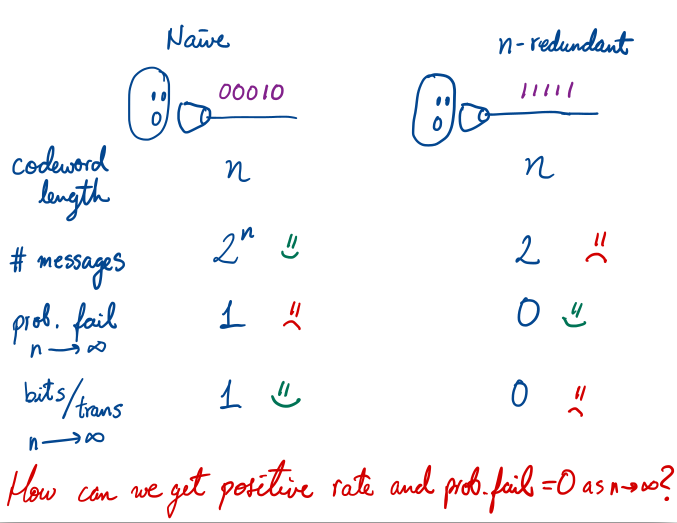
\includegraphics[width=\textwidth]{\dir/comparison_naive_n_redundant.png}
\caption{}
\label{fig:comparison_naive_n_redundant}
\end{figure}

\subsubsection*{Intuition on Shannon's channel coding theorem}

We started by using the binary noisy channel to send bits and we are now devising codes to send a finite set of letters through the binary noisy channel. In a similar manner, we can devise codes to send words through the binary noisy channel, by creating a code that maps words to bit strings of fixed length.
%\carlos{Why are we talking only of finite sentences $S$? In practice, I want to send sentences of variable lengths. Also, why don't we allow encodings of different lengths?} 

We can continue in this way to create codes to send images of a fixed size, videos of a fixed length, and so on.%\carlos{Why the obsession with fixed size?} 
All this is done by using longer codewords. 

%Observe, however, that the length $n$ of a codeword must be sufficiently large in order to
%%
%\begin{itemize}
%\item have a one-to-one correspondence from messages to codewords\carlos{What's a message?} and
%\item ensure robustness against the channel's noise.
%\end{itemize}
%%
%At the same time, the length $n$ of a codeword must not be too large, as the rate of actual bits of information per tranmission goes to $0$ as $n$ increases.

Shannon's coding theorem concerns with the problem of finding sustainable strategies for building codes. By sustainable, we mean that the strategy should yield codes that fulfill two conditions. 
%
\begin{itemize}
\item First, the codes attain and maintain a positive rate $r$ of bits of information per transmission as $n \to \infty$.
\item Second, the probability of a communication error goes to zero as $n \to \infty$.
\end{itemize}

Shannon's channel coding theorem states that there is a sustainable strategy for building codes, as long as the targeted rate $r$ is below the channel's capacity. For a fixed codeword length $n$, the maximum number of messages that can be communicated with this strategy is $\lfloor 2^{nr}\rfloor$.

\subsubsection*{Formalization}

For the definitions below, let $M, n \in \mathbb{N}$ and let $(\mathfrak{A}, \mathcal{P})$ be a channel.

\begin{definition}
An \emph{$(M, n)$-code} is a pair $(\mathit{Enc}, \mathit{Dec})$ of functions with $\mathit{Enc}: \{1, 2, \ldots, M\} \to \mathfrak{A}^n$ and $\mathit{Dec}: \mathfrak{A}^n \to \{1, 2, \ldots, M\}$.
\end{definition}

\begin{definition}
The \emph{rate of a $(M, n)$-code} is 
%
$$\frac{\log M}{n},$$
%
where the logarithm is in base 2.
\end{definition}

Observe that if a $(M, n)$-code has rate $r$, then $M = 2^{nr}$.

\begin{definition}
For an $(M, n)$-code $(\mathit{Enc}, \mathit{Dec})$,
its \emph{probability of a communication error} is
%
$$\frac{1}{M}\sum_{i \leq M} \prob\left(\mathit{Dec}(\hat{W}) \neq i \mid W = \mathit{Enc}\left(i\right)\right),$$
%
where $\prob\left(\mathit{Dec}(\hat{W}) \neq i \mid W = \mathit{Enc}\left(i\right)\right)$ is the probability that the receiver decodes something different to $i$, given that we sent $\mathit{Enc}\left(i\right)$ through the channel.
\end{definition}

Intuitively, the probability of a communication error is the probability that the receiver decodes a wrong message when we send him the codeword of a message chosen uniformly at random.

\begin{example}
The $n$-redundant code discussed above is an example of a $(2, n)$-code, whose rate is $\log 2 / n = 1/n$. In contrast, the na\"ive code is an example of a $(2^n, n)$-code, whose rate is $\log 2^n / n = 1$.
\end{example}

\begin{definition}
A rate $r$ is \emph{attainable} if there is a sequence of $\left(\lfloor2^{nr}\rfloor, n\right)$-codes, indexed by $n$, such that the probability of a communication error goes to zero as $n \to \infty$.
\end{definition}

\subsection{Shannon's coding theorem}

\subsubsection*{Typicality}

We now recall some important notions from Thomas and Cover~\cite{infotheory}

\begin{theorem}{(The asymptotic equipartition property)} Let $S, S_1$, $S_2, \ldots$, $S_n$ be identically and independently distributed random variables with distribution $p(\cdot)$ over a space $\mathcal{S}$, then
%
$$-\frac{1}{n} \log p(S_1, \ldots, S_n) \to H(S), \quad \text{in probability as } n \to \infty.$$
%
\end{theorem}

This theorem follows from the weak law of large numbers. In our context, $S, S_1, S_2, \ldots, S_n$ denote symbols from a channel's alphabet and $p(\cdot)$ is $\arg\max_p I(S; \hat{S})$. That is, $p(\cdot)$ is the distribution that achieves the channel's capacity.

\begin{definition}
For $n \in \mathbb{N}$ and $\epsilon > 0$, the \emph{typical set $A^{(n)}_\epsilon$} with respect to $p(\cdot)$ is the set of sequences $(s_1, \dots, s_n) \in \mathcal{S}^n$ such that
%
$$H(S) - \epsilon \leq -\frac{1}{n}\log p(s_1, s_2, \ldots, s_n) \leq H(S) + \epsilon.$$
%
A sequence in $A^{(n)}_\epsilon$ is called a \emph{typical sequence}.
\end{definition}

In our context, codewords will consist of typical sequences.
The next theorem justifies the following intuitions:

\begin{enumerate}
\item All typical sequences have approximately the same probability $\approx 2^{-nH(S)}$.
\item If you draw a sequence in $\mathcal{S}^n$, using $p(\cdot)$, then the resulting sequence is typical with high probability.
\item $\left|A^{(n)}_\epsilon\right| \approx 2^{nH(S)}$.
\end{enumerate}

\begin{theorem}\mbox{   }
\begin{enumerate}
\item If $\left(s_1, s_2, \ldots, s_n\right) \in A^{(n)}_\epsilon$, then $2^{-n\left(H(S) + \epsilon\right)} \leq p(s_1, \ldots, s_n) \leq 2^{-n\left(H(S) - \epsilon\right)}.$
\item $\prob\left(A^{(n)}_\epsilon\right) > 1 - \epsilon$, for sufficiently large $n$.
\item $(1 - \epsilon)2^{n\left(H(S) - \epsilon\right)} \leq \left|A^{(n)}_\epsilon\right| \leq 2^{n\left(H(S) + \epsilon\right)}$.
\end{enumerate}
\end{theorem}

The reader can take it as an exercise to proof these claims. The proofs are in Thomas and Cover~\cite{infotheory}.

\begin{definition}
Let $n \in \mathbb{N}$ and let $p_{S\hat{S}}(\cdot, \cdot)$ be the joint distribution of two random variables $S$ and $\hat{S}$, whose ranges are $\mathcal{S}$ and $\mathcal{\hat{S}}$, respectively. The set $A^{(n)}_\epsilon$ of \emph{jointly typical sequences} with respect to $p_{S\hat{S}}$ is the set of pairs $(\mathbf{s}^n, \hat{\mathbf{s}}^n)$ of sequences that fulfill the following:
%
\begin{enumerate}
\item $\left|-\frac{1}{n}\log p_{S^n}(\mathbf{s}^n) - H(S)\right| < \epsilon$.
\item $\left|-\frac{1}{n}\log p_{\hat{S}^n}(\hat{\mathbf{s}}^n) - H(\hat{S})\right| < \epsilon$.
\item $\left|-\frac{1}{n}\log p_{S^n\hat{S}^n}(\mathbf{s}^n, \hat{\mathbf{s}}^n) - H(S, \hat{S})\right| < \epsilon$.
\end{enumerate}
% 
A pair in $A^{(n)}_\epsilon$ is called a \emph{jointly typical pair of sequences}.
\end{definition}

We clarify that, for $\mathbf{s}^n = (s_1, \ldots, s_n)$ and $\hat{\mathbf{s}}^n = (\hat{s}_1, \ldots, \hat{s}_n)$,
%
$$p_{S^n}(\mathbf{s}^n) = \prod_{i \leq n} p_S(s_i),$$
%
$$p_{\hat{S}^n}(\hat{\mathbf{s}}^n) = \prod_{i \leq n} p_{\hat{S}}(\hat{s}_i) = \prod_{i \leq n} \sum_{s} p_S(s) p_{\hat{S}\mid S}\left(\hat{s}_i \mid s\right), \text{and}$$
%
$$p_{S^n\hat{S}^n}(\mathbf{s}^n, \hat{\mathbf{s}}^n) = \prod_{i \leq n} p_{S\hat{S}}(s_i, \hat{s}_i) = \prod_{i \leq n} p_S(s_i) p_{\hat{S} \mid S}(\hat{s}_i \mid s_i).$$

In the context of communication via a channel, $p_{S^n\hat{S}^n}$ represents the joint distribution of $\mathbf{S}^n$ and $\hat{\mathbf{S}}^n$, where 
%
\begin{itemize}
\item $\mathbf{S}^n$ denotes a random codeword, where each symbol was chosen at random according to the distribution $p_S = \arg \max_p I(S; \hat{S})$ that achieves channel capacity.
\item $\hat{\mathbf{S}}^n$ denotes a codeword that the channel would output, after we send $\mathbf{S}^n$ as input.
\end{itemize}
%
We call $p_{S^n\hat{S}^n}$ the \emph{codeword input-output distribution}.

In the context of communication via a channel, the following theorem justifies the following intuitions:

\begin{enumerate}
\item Suppose that we build a codeword $\mathbf{s}^n$ at random by choosing each of its symbols at random according to $p_S$, the distribution that attains channel capacity. Then we send $\mathbf{s}^n$ through the channel and let $\hat{\mathbf{s}}^n$ be the output codeword. Then $(\mathbf{s}^n, \hat{\mathbf{s}}^n)$ is jointly typical with high probability.
\item Suppose now that we build another codeword ${\mathbf{q}}^n$ at random by choosing each of its symbols at random according to $p_S$. Then it is very \emph{unlikely} that $({\mathbf{q}}^n,\hat{\mathbf{s}}^n)$ is jointly typical.
\end{enumerate}

\begin{theorem}\mbox{  }
\begin{enumerate}
\item $\prob\left(\left(\mathbf{S}^n, \hat{\mathbf{S}}^n\right) \in A^{(n)}_{\epsilon}\right) \to 1$, as $n \to \infty$.
\item If $\mathbf{Q}^n \sim p_{S^n}(\cdot)$ and $\hat{\mathbf{S}}^n \sim p_{\hat{S}^n}(\cdot)$ (i.e., they are drawn independently at random from the marginal distributions of $p_{S^n\hat{S}^n}$), then
%
$$(1-\epsilon)2^{-n\left(I(S;\hat{S}) + 3\epsilon\right)} \leq \prob\left(\left({\mathbf{Q}}^n, \hat{\mathbf{S}}^n\right) \in A^{(n)}_{\epsilon}\right) \leq 2^{-n\left(I(S;\hat{S}) - 3\epsilon\right)}$$
%
\end{enumerate}
\label{thm:joint_typical}
\end{theorem}

These two intuitions justify the effectiveness of a very simple code, called \emph{Shannon's random code}. 

\subsubsection*{Shannon's random code}

\begin{theorem}
A rate is attainable iff it is below the channel's capacity.
\end{theorem}

We only focus here on proving the following direction: if a rate is below the channel's capacity, then it is attainable, as it illustrates how to propose a $(\lfloor 2^{nr} \rfloor, n)$-code for communicating $\lfloor 2^{nr} \rfloor$ messages.

To prove this, we present, for $n > 1$, a $(\lfloor 2^{nr}\rfloor, n)$-code whose probability of a communication error is at most $p_n = 2^{-n\left(\mathit{cap} - 3\epsilon - r\right)}$, where $\epsilon$ is chosen to be sufficiently small. Hence, if $r < \mathit{cap}$, we get that the probability of a communication error goes to zero as $n \to \infty$.

The code's encoder function $\mathit{Enc}$ is defined as follows. For a message $m \leq \lfloor 2^{nr}\rfloor$, we define $\mathit{Enc}(m)$ as a string in $\mathbf{s}^n$ where each symbol was drawn from a distribution $p^* = \arg\max_{p(\cdot)} I(S; \hat{S})$. That is, a distribution that maximizes the channel's input-output mutual information and attains the channel's capacity.

The code's decoder function $\mathit{Dec}$ is defined as follows. Given the string $\hat{\mathbf{s}}^n$ output by the channel, $\mathit{Dec}$ goes through each message $m$ and tests if $(\mathit{Enc}(m), \hat{\mathbf{s}}^n)$ is jointly typical with respect to the codeword input-output distribution $p_{S^n\hat{S}^n}$. $\mathit{Dec}$ outputs the first message for which this test succeeds. If no message succeeds on the test, then $\mathit{Dec}$ outputs an arbitrary message.

%\carlos{Remind the reader that the sender and the receiver agree in advance on $\mathit{Enc}$ and $\mathit{Dec}$. Therefore, the receiver also knows both $\mathit{Enc}$ and the set $\{1, 2, \ldots, \lfloor 2^{nr}\rfloor$ of messages.}

\begin{theorem}
The probability $\prob\left(\mathcal{E}\right)$ of a communication error for Shannon's random code goes to 0 as $n \to \infty$.
\label{thm:shannon_random_code}
\end{theorem}

\begin{proof}
Let $\mathcal{K}$ be a random variable representing a possible code. Then
%
$$\prob\left(\mathcal{E}\right) = \sum_{\mathcal{K}} \prob\left(\mathcal{K}\right) P_e(\mathcal{K}),$$
%
where $P_e(\mathcal{K})$ is the probability of a communication error for code $\mathcal{K}$. Observe now that
%
\begin{align*}
\prob\left(\mathcal{E}\right) &= \sum_{\mathcal{K}} \prob\left(\mathcal{K}\right) P_e(\mathcal{K})\\
&= \sum_{\mathcal{K}} \prob\left(\mathcal{K}\right) \frac{1}{\lfloor 2^{nr}\rfloor}\sum_{w \leq \lfloor 2^{nr}\rfloor} \prob\left(\mathit{Dec}(\hat{\mathbf{S}}^n) \neq w \mid \mathbf{S}^n = \mathit{Enc}(w)\right)\\
&= \frac{1}{\lfloor 2^{nr}\rfloor} \sum_{\mathcal{K}} \sum_{w \leq \lfloor 2^{nr}\rfloor} \prob\left(\mathcal{K}\right)  \prob\left(\mathit{Dec}(\hat{\mathbf{S}}^n) \neq w \mid \mathbf{S}^n = \mathit{Enc}(w)\right).
\end{align*}

Observe now that all codewords were chosen independently at random, so 
%
$$\prob\left(\mathit{Dec}(\hat{\mathbf{S}}^n) \neq w \mid \mathbf{S}^n = \mathit{Enc}(w)\right) = \prob\left(\mathit{Dec}(\hat{\mathbf{S}}^n) \neq 1 \mid \mathbf{S}^n = \mathit{Enc}(1)\right),$$ 
%
for $w > 1$. Hence,
%
\begin{align*}
\prob\left(\mathcal{E}\right) &= \frac{1}{\lfloor 2^{nr}\rfloor} \sum_{\mathcal{K}} \sum_{w \leq \lfloor 2^{nr}\rfloor} \prob\left(\mathcal{K}\right)  \prob\left(\mathit{Dec}(\hat{\mathbf{S}}^n) \neq w \mid \mathbf{S}^n = \mathit{Enc}(w)\right)\\
&= \sum_{\mathcal{K}} \prob\left(\mathcal{K}\right)  \prob\left(\mathit{Dec}(\hat{\mathbf{S}}^n) \neq 1 \mid \mathbf{S}^n = \mathit{Enc}(1)\right)\\
&= \prob\left(\mathcal{E} \mid w = 1\right).
\end{align*}

This means that the probability of a communication error is equal to the probability of a communication error, assuming that the sender sent the codeword for message 1.

Note that, in Shannon's random code, the event of a communication error implies at least one of the following events: the received codeword $\hat{\mathbf{S}}^n(1)$ is not jointly typical with the codeword $\mathbf{S}^n(1)$ for message 1 or the received codeword $\hat{\mathbf{S}}^n(1)$ is jointly typical with the codeword $\mathbf{S}^n(w)$ for a message $w > 1$. More precisely,
%
\begin{align*}
\prob\left(\mathcal{E} \mid M = 1\right) &= \prob\left(
\begin{array}{c}
\left(\mathbf{S}^n(1), \hat{\mathbf{S}}^n(1)\right) \notin A^{(n)}_{\epsilon} \; \text{or}\\
\left(\mathbf{S}^n(2), \hat{\mathbf{S}}^n(1)\right) \in A^{(n)}_{\epsilon} \; \text{or}\\
\left(\mathbf{S}^n(3), \hat{\mathbf{S}}^n(1)\right) \in A^{(n)}_{\epsilon} \; \text{or}\\
\vdots\\
\left(\mathbf{S}^n(\lfloor2^{nr}\rfloor), \hat{\mathbf{S}}^n(1)\right) \in A^{(n)}_{\epsilon}.
\end{array}
\right).
\end{align*}
%
By the union bound,
%
$$\prob\left(\mathcal{E} \mid M = 1\right) \leq \prob\left(\left(\mathbf{S}^n(1), \hat{\mathbf{S}}^n(1)\right) \notin A^{(n)}_{\epsilon}\right) + \sum_{w > 1}\prob\left(\left(\mathbf{S}^n(w), \hat{\mathbf{S}}^n(1)\right) \in A^{(n)}_{\epsilon}\right).$$
%
We now apply Theorem~\ref{thm:joint_typical}, which implies the following:

\begin{itemize}
\item $\prob\left(\left(\mathbf{S}^n(1), \hat{\mathbf{S}}^n(1)\right) \in A^{(n)}_{\epsilon}\right) \to 1$, as $n \to \infty$. In other words, $\prob\left(\left(\mathbf{S}^n(1), \hat{\mathbf{S}}^n(1)\right) \notin A^{(n)}_{\epsilon}\right) \to 0$, as $n \to \infty$.
\item $\prob\left(\left(\mathbf{S}^n(w), \hat{\mathbf{S}}^n(1)\right) \in A^{(n)}_{\epsilon}\right) \leq 2^{-n\left(I(S;\hat{S})-3\epsilon\right)}$. This is because, for $w > 1$, $\mathbf{S}^n(1)$ and $\mathbf{S}^n(w)$ were independently drawn from $p_{S^n}$ and, therefore, $\hat{\mathbf{S}}^n(1)$ and $\mathbf{S}^n(w)$ were independently drawn from $p_{\hat{S}^n}$ and $p_{S^n}$, respectively.
\end{itemize}

Using these observations we get that
%
\begin{align*}
\prob\left(\mathcal{E} \mid M = 1\right) &\leq \prob\left(\left(\mathbf{S}^n(1), \hat{\mathbf{S}}^n(1)\right) \notin A^{(n)}_{\epsilon}\right) + \sum_{w > 1}\prob\left(\left(\mathbf{S}^n(w), \hat{\mathbf{S}}^n(1)\right) \in A^{(n)}_{\epsilon}\right)\\
&\leq \prob\left(\left(\mathbf{S}^n(1), \hat{\mathbf{S}}^n(1)\right) \notin A^{(n)}_{\epsilon}\right) + \sum_{w > 1} 2^{-n\left(I(S;\hat{S}) - 3\epsilon\right)}\\
&= \prob\left(\left(\mathbf{S}^n(1), \hat{\mathbf{S}}^n(1)\right) \notin A^{(n)}_{\epsilon}\right) + \left(\lfloor 2^{nr}\rfloor - 1\right)2^{-n\left(I(S;\hat{S}) - 3\epsilon\right)}\\
&\leq \prob\left(\left(\mathbf{S}^n(1), \hat{\mathbf{S}}^n(1)\right) \notin A^{(n)}_{\epsilon}\right) + 2^{nr} 2^{-n\left(I(S;\hat{S}) - 3\epsilon\right)}\\
&= \prob\left(\left(\mathbf{S}^n(1), \hat{\mathbf{S}}^n(1)\right) \notin A^{(n)}_{\epsilon}\right) + 2^{-n\left(I(S;\hat{S}) - r - 3\epsilon\right)}.
\end{align*}
%

Observe that we chose $p_S$ as $\arg\max_p I(S;\hat{S})$, so $I(S;\hat{S}) = \mathit{cap}$, the channel's capacity. So, if the rate $r$ is below the channel's capacity and $\epsilon$ is sufficiently small, then $\prob\left(\mathcal{E} \mid M = 1\right) \to 0$ as $n \to \infty$.
\end{proof}

\section{Communication protocol for algorithm validation}
\label{sec:comm_protocol}

We now formalize the communication protocol where posterior agreement originates. We first explain an \emph{ideal variant} where we know $X$'s probability distribution $p_X$. Furthermore, we assume that $p_X$ is from a parameterized family $\mathfrak{P}$ of probability distributions. Afterwards, we explain the \emph{empirical variant} where we do not know anything about $p_X$ and, even worse, we only have \emph{two observations} $X'$ and $X''$ drawn from $p_X$. Recall that, in practice, we only have access to observations and have no information of the nature of the distribution where these observations came from.\looseness=-1

\subsection{Assumptions}

For our statements to hold, we make the following assumptions.

\paragraph{Exponential solution space:} We assume that $\mathcal{C}$ is discrete and that $\log \left|\mathcal{C}\right| = \Theta(n)$, where $n$ measures the ``size'' of an observation from a phenomenon. For example, $n$ measures the number of edges in a graph or the number of datapoints in a clustering instance. Intuitively, we assume that the solution space's size grows exponentially in $n$.

\paragraph{Probabilistic outputs:} We assume that any algorithm for stochastic optimization, when given an input $X'$ from an instance space $\mathcal{X}$, outputs a distribution $p(\cdot \mid X')$ over a discrete solution space $\mathcal{C}$. Every algorithm can be thought to be as such, even when it only outputs a fixed value $c_{X'} \in \mathcal{C}$, when given $X'$ as input. In this case, $p(c \mid X') = 1$ if $c = c_{X'}$ and $0$ otherwise.

\subsection{Ideal variant}

Let $\mathcal{A}$ be an algorithm intended for solving Problem~\ref{eq:stoch_min_span_tree}. Posterior agreement originates from a communication protocol between a sender and a receiver. The sender must communicate, using $\mathcal{A}$'s outputs, the nature of a phenomenon to the receiver. The receiver must be able, using the information sent from the sender, to identify the phenomenon. The communication from the sender to the receiver is done through a noisy channel, whose noise is defined by $\mathcal{A}$ and the phenomenon.

\paragraph{Messages} Fix $n \in \mathbb{N}$. Present the instance space $\mathcal{X}$ to the sender and the receiver. Then agree draw at random a set $\mathcal{F} \subseteq \mathfrak{P}$ of $m$ phenomena and, for each $p_i \in \mathcal{F}$, draw an observation $X'_i$ of size $n$. Let $\mathcal{M} = \{X'_1, \ldots, X'_m\}$. Agreeing on $\mathcal{F}$ is often not possible in practice, so we explain in the empirical variant how to deal with this. This $\mathcal{M}$ constitutes the set of possible messages that the sender may try to communicate to the receiver.

For the moment, we leave the value of $m$ undefined. We leave for later to figure out what is the maximum value of $m$ that we can use. The choice of $m$ must still ensure that the probability of a communication error goes to 0, as $n \to \infty$.

\paragraph{Code} Present algorithm $\mathcal{A}$ to the sender and the receiver. For each $X' \in \mathcal{M}$, use $\mathcal{A}$ to compute $p(\cdot \mid X')$. Define the code $(\mathit{Enc}_{\mathcal{A}}, \mathit{Dec}_{\mathcal{A}})$ as follows:

\begin{itemize}
\item $\mathit{Enc}_{\mathcal{A}}$ encodes $X' \in \mathcal{M}$ as the codeword $p(\cdot \mid X')$.
\item $\mathit{Dec}_{\mathcal{A}}$ decodes a probability distribution $p(\cdot \mid Y)$ over $\mathcal{C}$ as any $\hat{X} \in \mathcal{M}$ such that $\kappa\left(Y, \hat{X}\right) \geq \kappa\left(Y, X\right)$, for all $X \in \mathcal{M}$. Here,
%
$$\kappa\left(Y, X'\right) := \sum_c p(c \mid Y)p(c \mid X').$$
%
\end{itemize}

\paragraph{Channel} The channel is the pair $\left(\left\{p(\cdot \mid X')\right\}_{X' \in \mathcal{M}}, \mathcal{P}\right)$ where $\mathcal{P}$ is defined by the following probabilistic procedure. Assume that the sender inputs $p(\cdot \mid X')$ to the channel. The channel then replaces $X'$ with a fresh new observation $X''$ from the same phenomenon where $X'$ comes from. Then it uses the algorithm $\mathcal{A}$ to compute $p(\cdot \mid X'')$ and outputs that to the receiver.

\paragraph{Communication} A message $X'$ is selected uniformly at random from $\mathcal{M}$ and without the receiver's knowledge. The sender then sends the codeword $p(\cdot \mid X')$ through the channel. The receiver gets $p(\cdot \mid X'')$ and uses the decoding function to guess which message the sender sent. The receiver succeeds by correctly guessing the phenomenon from where $X'$ was drawn from.

Observe how the algorithm and the phenomenon define the channel's noise. Hence, the algorithm can be evaluated by \emph{the capacity} of the resulting channel. This capacity is measured by its maximum attainable rate, which is obtained by figuring out how to maximize the number $m$ of messages that can be used in the protocol, while making the probability of a communication error go to zero as $n$, the size of the observations, go to infinity. We carry this analysis in the empirical variant.

\subsection{Empirical variant}

The capacity of the channel built above cannot be computed, as we often only have access to a set of observations and not to the phenomena behind them. This means that we cannot compute the set $\mathcal{M}$ of messages, as described in the ideal variant. For this reason, we use an empirical variant, where we assume that we are given at least two observations $X'$ and $X''$ of a same phenomenon.

\paragraph{Messages} (Figure~\ref{fig:agree_on_trans}) We create a set of messages by producing \emph{transformed copies} of $X'$. We take a set $\mathbb{T}$ of transformations, where each transformation transforms instances into instances. Afterwards, we draw $m$ transformations  $\tau_1, \tau_2, \ldots, \tau_m$ from $\mathbb{T}$ uniformly at random. In this way, we can create a set $\mathcal{M} = \left\{\tau_1 \circ X', \tau_2 \circ X', \ldots, \tau_m \circ X'\right\}$ of messages that are analogous to the set of messages that we created in the ideal variant. We impose the following requirements on $\mathbb{T}$ so that $\mathcal{M}$ looks like the set $\mathcal{M}$ that we would obtain in the ideal variant.

\begin{itemize}
\item $\sum_{\tau} p(c \mid \tau \circ X') \in \left[\frac{\left|\mathbb{T}\right|}{\left|\mathcal{C}\right|}(1 - \rho), \frac{\left|\mathbb{T}\right|}{\left|\mathcal{C}\right|}(1 + \rho)\right]$, for some small $\rho > 0$. The reason for this assumption is that we we do not want the probability mass of all these codewords to be concentrated in a narrow subset of $\mathcal{C}$, as this reduces the number of different messages that the sender can communicate to the receiver. This ensures that, for each $c \in \mathcal{C}$, the total probability mass $c$ gets is $\sum_{\tau} p(c \mid \tau \circ X') \approx \frac{\left|\mathbb{T}\right|}{\left|\mathcal{C}\right|}$.
\item The transformations do not alter an instance's randomness. 
%\item For any $\tau_1, \tau_2 \in \mathbb{T}$, $\left|p(\cdot \mid \tau_1 \circ X') - p(\cdot \mid \tau_2 \circ X'')\right| > 0$. That is, different transformations should induce different codewords.
\end{itemize}

Observe that such a set of transformations does not necessarily always exist. For example, if the algorithm under evaluation always produces the same constant distribution $p(\cdot \mid X')$, independent of $X'$, then no set of transformations will be able to achieve the requirement above. In this case, however, there is no need to build a channel to evaluate such an algorithm, as it is clear that the algorithm is not producing any value from the data.

\begin{figure}
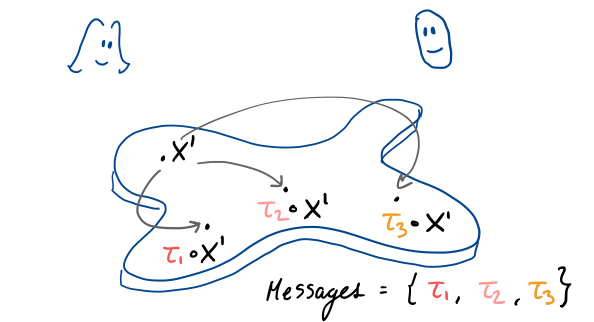
\includegraphics[width=\textwidth]{\dir/agree_on_trans.png}
\caption{}
\label{fig:agree_on_trans}
\end{figure}

\paragraph{Code} (Figure~\ref{fig:emp_agree_on_code}) The encoding and decoding functions are the analogous of the ideal variant. The codeword of a message $\tau \in \mathcal{M}$ is $p(\cdot \mid \tau \circ X')$. When given a codeword $p(\cdot \mid Y)$, the decoding function outputs the message $\tau$ for which $\kappa\left(Y, \tau \circ X'\right) \geq \kappa\left(Y, \sigma \circ X'\right)$, for every $\sigma \in \mathcal{M}$.

\begin{figure}
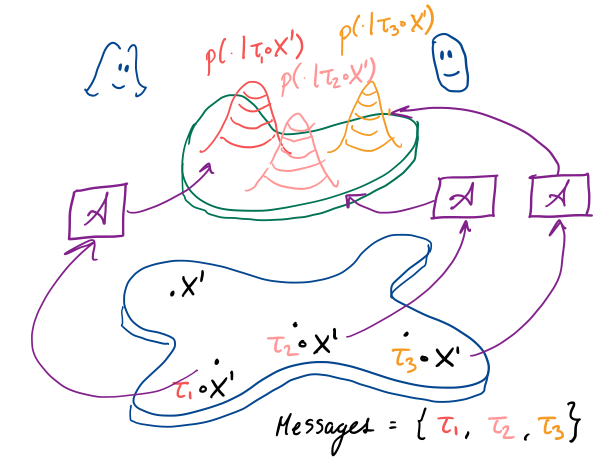
\includegraphics[width=\textwidth]{\dir/emp_agree_on_code.png}
\caption{}
\label{fig:emp_agree_on_code}
\end{figure}

\paragraph{Channel} (Figure~\ref{fig:send_codeword}) When the sender inputs $p(\cdot \mid \tau \circ X')$ to the channel, the channel outputs $p(\cdot \mid \tau \circ X'')$, as in the ideal variant.

\begin{figure}
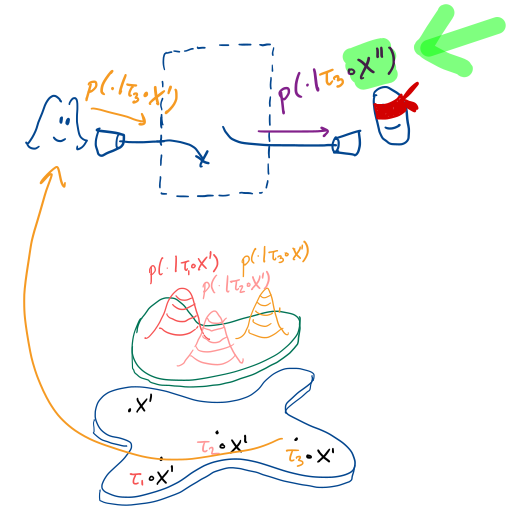
\includegraphics[width=\textwidth]{\dir/send_codeword.png}
\caption{}
\label{fig:send_codeword}
\end{figure}

\paragraph{Protocol} The sender and the receiver agree on a set $\mathbb{T}$ of transformations and use the algorithm under evaluation $\mathcal{A}$ to compute the code's encoding and decoding functions. A set $\mathcal{M} = \left\{\tau_1, \ldots, \tau_m\right\}$ of $m$ messages is drawn uniformly at random from $\mathbb{T}$. A message $\tau \in \mathcal{M}$ is selected uniformly at random and without the receiver's knowledge. The sender then sends the codeword $p(\cdot \mid \tau \circ X')$ through the channel. The receiver gets $p(\cdot \mid \tau \circ X'')$ and uses the decoding function to guess which message the sender sent (Figure~\ref{fig:guessing}). The receiver succeeds by correctly guessing $\tau$.

\begin{figure}
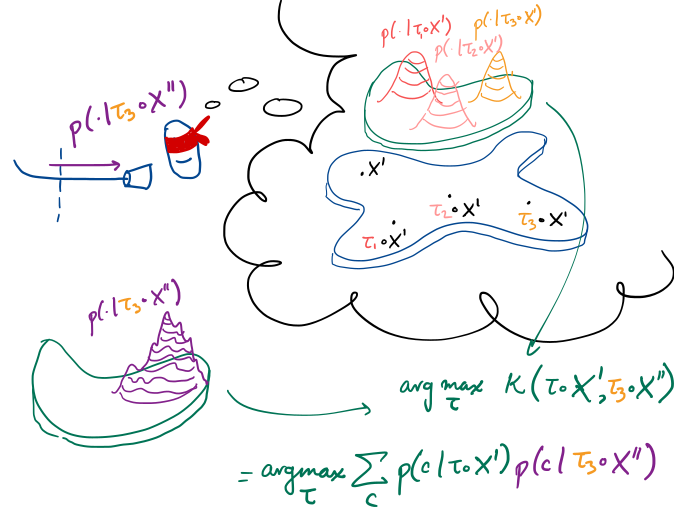
\includegraphics[width=\textwidth]{\dir/emp_guessing.png}
\caption{}
\label{fig:emp_guessing}
\end{figure}

\subsection{Probability of a communication error}
\label{sub:prob_comm_error}

\begin{definition}
The \emph{expected log posterior agreement kernel of an algorithm} is $\mathcal{E} := \mathbb{E}_{X', X''}\left[\log \kappa\left(X', X''\right)\right]$.
\end{definition}

\begin{definition}
An algorithm fulfils \emph{the asymptotic equipartition property (AEP)} if
$\log \kappa\left(X', X''\right)$ converges in probability to $\mathcal{E}$, as $n \to \infty$, where $n$ is the size of $X'$.
\end{definition}

\begin{definition}
For $\epsilon > 0$ and $n \in \mathbb{N}
$, the \emph{set $A^{(n)}_\epsilon$ of $(\epsilon, n)$-typical pairs} consists of all pairs $X', X''$ of instances of size $n$ such that
%
\begin{equation}
\left|\log \kappa\left(X', X''\right) -  \mathcal{E}\right| < \epsilon.
\end{equation}
%
\end{definition}

\begin{exercise}
Show that as $n \to \infty$, $\log\kappa\left(X', X''\right)$ is very close to $\mathcal{E}$ with high probability. That is, show that for any $\epsilon > 0$, there is a sufficiently large $N$, such that for any $n \geq N$, $\prob\left(A^{(n)}_\epsilon\right) \geq 1 - \epsilon$.
\label{ex:almost_all_typical_pa}
\end{exercise}

\begin{exercise}
Show that as $n \to \infty$, one can ignore those pairs $X', X''$ for which $\kappa\left(X', X''\right)$ is negligible. That is, show that for any $\epsilon > 0$, there is a sufficiently large $N$, such that for any $n \geq N$,
%
\begin{equation}
\prob\left(\kappa\left(X', X''\right) < 2^{(\mathcal{E} - \epsilon)}\right) < \epsilon.
\end{equation}
%
\label{ex:ignore_negligible_pa}
\end{exercise}

\begin{theorem}
Assume given an algorithm that fulfils the AEP.
For $\epsilon > 0$, there is a sufficiently large $N$, such that for any $n \geq N$, the probability of a communication error is bounded above by 
%
\begin{equation}
P_{(n)} = \left(1 + \rho\right)\exp\left(-\log\left|\mathcal{C}\right|\left(I - \frac{\log m}{\log \left|\mathcal{C}\right|} -  \frac{\epsilon}{m\log \left|\mathcal{C}\right|}\right)\right) + 2^{\epsilon - \mathcal{E}}\frac{\left(1 + \rho\right)\epsilon}{\left|\mathcal{C}\right|},
\label{eq:prob_comm_error_empirical_var}
\end{equation}
%
where
%
\begin{equation}
I := \frac{1}{\log\left|\mathcal{C}\right|}\mathbb{E}_{X', X''}\left[\log \left(\left|\mathcal{C}\right|k(X', X'')\right)\right]
\label{eq:exp_log_pa}
\end{equation}
%
\label{thm:comm_error_emp_var}
\end{theorem}

One can show that $P_{(n)} \to 0$ as $n \to \infty$ by choosing $\epsilon$ sufficiently small and ensuring that $I - \frac{\log m}{\log \left|\mathcal{C}\right|} > 0$.

\begin{proof}
Let $\epsilon > 0$. We assume that $\kappa\left(X', X''\right) \geq 2^{(\mathcal{E} - \epsilon)}$ for all pairs $X', X''$ of instances of size $n$. The proof is easily adapted to the more general case, by using Exercise~\ref{ex:ignore_negligible_pa}. This is left as an exercise.

Let $\tau_s$ be the message sent by the sender and let $\hat{\tau}$ be the message guessed by the receiver. Just as in the proof of Theorem~\ref{thm:shannon_random_code}, one can show that $\prob\left(\hat{\tau} \neq \tau_s\right) = \prob\left(\hat{\tau} \neq \mathit{id}\right)$, where $\mathit{id}$ is some arbitrary transformation. Without loss of generality, we assume that $\mathit{id}$ is the identity transformation.

Using the definition of communication error, we get that
%
$$\prob\left(\hat{\tau} \neq \mathit{id}\right) = \prob\left(\max_{\tau \neq \mathit{id}} \kappa\left(\tau\circ X', X''\right) \geq \kappa\left(X', X''\right) \mid \mathit{id}\right).$$
%
Applying the union bound, we get
%
$$\prob\left(\hat{\tau} \neq \mathit{id}\right) \leq \sum_{\tau \neq \mathit{id}}\prob\left(\kappa\left(\tau\circ X', X''\right) \geq \kappa\left(X', X''\right) \mid \mathit{id}\right).$$
%
We now rewrite probabilities as expectations
%
\begin{align*}
\prob\left(\hat{\tau} \neq \mathit{id}\right) &\leq \sum_{\tau \neq \mathit{id}}\prob\left(\kappa\left(\tau\circ X', X''\right) \geq \kappa\left(X', X''\right) \mid \mathit{id}\right)\\
&= \sum_{\tau \neq \mathit{id}}\mathbb{E}_{X', X''}\left[\mathbb{E}_{\tau}\left[\mathbb{I}\left\{\kappa\left(\tau\circ X', X''\right) \geq \kappa\left(X', X''\right)\right\} \mid \mathit{id}, X', X''\right]\right]\\
&= \sum_{\tau \neq \mathit{id}}\mathbb{E}_{X', X''}\left[\prob\left(\kappa\left(\tau\circ X', X''\right) \geq \kappa\left(X', X''\right) \mid \mathit{id}, X', X''\right)\right].
\end{align*}
%
Here, $\mathbb{I}$ is the indicator function.

We now apply Markov's inequality.
%
\begin{align*}
\prob\left(\hat{\tau} \neq \mathit{id}\right) &\leq \sum_{\tau \neq \mathit{id}}\mathbb{E}_{X', X''}\left[\prob\left(\kappa\left(\tau\circ X', X''\right) \geq \kappa\left(X', X''\right) \mid \mathit{id}, X', X''\right)\right]\\
&\leq \sum_{\tau \neq \mathit{id}}\mathbb{E}_{X', X''}\left[\frac{\mathbb{E}_\tau\left[\kappa\left(\tau \circ X', X''\right) \mid \mathit{id}, X', X'' \right]}{\kappa\left(X', X''\right)}\right].
\end{align*}
%

We now compute an upper bound for the numerator.
%
\begin{align*}
\mathbb{E}_\tau \left[\kappa\left(\tau \circ X', X''\right) \mid X', X''\right]
&= \mathbb{E}_\tau \left[\sum_c p(c \mid \tau \circ X') p(c \mid X'') \mid X', X''\right]\\
&= \sum_c p(c \mid X'') \mathbb{E}_\tau \left[p(c \mid \tau \circ X')\right]\\
&= \sum_c p(c \mid X'') \sum_\tau \frac{1}{\left|\mathbb{T}\right|} p(c \mid \tau \circ X')\\
&\leq \frac{1}{\left|\mathbb{T}\right|}\frac{\left|\mathbb{T}\right|}{\left|\mathcal{C}\right|}(1 + \rho)\sum_c p(c \mid X'') = (1 + \rho)\frac{1}{\left|\mathcal{C}\right|}.
\end{align*}
%
For the last inequality, we used the assumption that $\sum_{\tau} p(c \mid \tau \circ X') \in \left[\frac{\left|\mathbb{T}\right|}{\left|\mathcal{C}\right|}(1 - \rho), \frac{\left|\mathbb{T}\right|}{\left|\mathcal{C}\right|}(1 + \rho)\right]$.

We have then that
%
\begin{align}
\prob\left(\hat{\tau} \neq \mathit{id}\right) &\leq \sum_{\tau \neq \mathit{id}} \mathbb{E}_{X', X''}\left[\frac{1 + \rho}{\left|\mathcal{C}\right|\kappa\left(X', X''\right)}\right]\\
&= \frac{\left(1 + \rho\right)(m - 1)}{\left|\mathcal{C}\right|}\mathbb{E}_{X', X''}\left[\frac{1}{\kappa\left(X', X''\right)}\right]\\
&\leq \frac{\left(1 + \rho\right)m}{\left|\mathcal{C}\right|}\mathbb{E}_{X', X''}\left[\frac{1}{\kappa\left(X', X''\right)}\right].\label{eq:curr_upp_bound}
\end{align}
%

Observe that pairs $X', X''$ where $\kappa\left(X', X''\right)$ are very low pose a serious threat to our attempt to bound $\prob\left(\hat{\tau} \neq \mathit{id}\right)$. Fortunately, by the AEP property, Exercises~\ref{ex:almost_all_typical_pa}, and our assumption that $\kappa(X', X'') \geq 2^{\mathcal{E} - \epsilon}$, we can ignore them as follows. Choose a sufficiently large $N$ so that, for any $n \geq N$, $\prob\left(X', X'' \notin A^{(n)}_{\epsilon/m}\right) < \epsilon / m$. Then
%
\begin{align}
\mathbb{E}_{X', X''}\left[\frac{1}{\kappa\left(X', X''\right)}\right]
&= \left(
\begin{array}{l}
\sum_{X', X'' \in A^{(n)}_{\epsilon/m}}p(X', X'')\frac{1}{\kappa\left(X', X''\right)} +\\ 
\sum_{X', X'' \notin A^{(n)}_{\epsilon/m}}p(X', X'')\frac{1}{\kappa\left(X', X''\right)}
\end{array}\right)\\
&\leq \left(
\begin{array}{l}
\sum_{X', X'' \in A^{(n)}_{\epsilon/m}}p(X', X'')\frac{1}{\kappa\left(X', X''\right)} +\\ 
2^{\epsilon - \mathcal{E}}\prob\left(X', X'' \notin A^{(n)}_{\epsilon/m}\right)
\end{array}\right)\\
&\leq \left(
\begin{array}{l}
\sum_{X', X'' \in A^{(n)}_{\epsilon/m}}p(X', X'')\frac{1}{\kappa\left(X', X''\right)} +\\ 
2^{\epsilon - \mathcal{E}}\frac{\epsilon}{m}
\end{array}\right)\\
&= \mathbb{E}_{X', X''}\left[\frac{1}{\kappa\left(X', X''\right)} \mid X', X'' \in A^{(n)}_{\epsilon/m}\right] + 2^{\epsilon - \mathcal{E}}\frac{\epsilon}{m}.
\end{align}

If we now substitute this into (\ref{eq:curr_upp_bound}), we get that
%
\begin{align}
\prob\left(\hat{\tau} \neq \mathit{id}\right) &\leq \frac{\left(1 + \rho\right)m}{\left|\mathcal{C}\right|}\left(\mathbb{E}_{X', X''}\left[\frac{1}{\kappa\left(X', X''\right)} \mid X', X'' \in A^{(n)}_{\epsilon/m}\right] + 2^{\epsilon - \mathcal{E}}\frac{\epsilon}{m}\right)\\
&= \frac{\left(1 + \rho\right)m}{\left|\mathcal{C}\right|}\mathbb{E}_{X', X''}\left[\frac{1}{\kappa\left(X', X''\right)} \mid X', X'' \in A^{(n)}_{\epsilon/m}\right] + 2^{\epsilon - \mathcal{E}}\frac{\left(1 + \rho\right)\epsilon}{\left|\mathcal{C}\right|}.\label{eq:semifinal_result}
\end{align}

We can rewrite the expectation as follows:

\begin{align}
&\frac{m}{\left\lvert\mathcal{C}\right\rvert} \mathbb{E}_{X', X''}\left[\frac{1}{\kappa\left(X', X''\right)} \mid X', X'' \in A^{(n)}_{\epsilon/m}\right]\\ 
&= \mathbb{E}_{X', X''}\left[\exp\left(- \log\kappa\left(X', X''\right) + \log m - \log \left|\mathcal{C}\right|\right) \mid X', X'' \in A^{(n)}_{\epsilon/m}\right]\\
&\leq \mathbb{E}_{X', X''}\left[\exp\left(- \mathcal{E} + \frac{\epsilon}{m} + \log m - \log \left|\mathcal{C}\right|\right) \mid X', X'' \in A^{(n)}_{\epsilon/m}\right]\\
&= \mathbb{E}_{X', X''}\left[\exp\left(-\log\left|\mathcal{C}\right|\left(I - \frac{\epsilon}{m\log \left|\mathcal{C}\right|} - \frac{\log m}{\log \left|\mathcal{C}\right|}\right)\right) \mid X', X'' \in A^{(n)}_{\epsilon/m}\right].
\end{align}

If we substitute this into~(\ref{eq:semifinal_result}), we get that $\prob\left(\hat{\tau} \neq \mathit{id}\right)$ is bounded above by

\begin{equation} \left(1 + \rho\right)\exp\left(-\log\left|\mathcal{C}\right|\left(I - \frac{\log m}{\log \left|\mathcal{C}\right|} -  \frac{\epsilon}{m\log \left|\mathcal{C}\right|}\right)\right) + 2^{\epsilon - \mathcal{E}}\frac{\left(1 + \rho\right)\epsilon}{\left|\mathcal{C}\right|}.
\end{equation}
This concludes the proof.
%
%
%\begin{align*}
%&= (1 + \rho)\left(m - 1\right) \mathbb{E}_{X', X''}\exp\left(-\log\left(\left|\mathcal{C}\right|\kappa\left(X', X''\right)\right)\right)\\
%&\leq m (1 + \rho) \; \mathbb{E}_{X', X''}\exp\left(-\log\left(\left|\mathcal{C}\right|\kappa\left(X', X''\right)\right)\right)\\
%&= (1 + \rho)\mathbb{E}_{X', X''}\exp\left(-\log\left(\left|\mathcal{C}\right|\kappa\left(X', X''\right)\right) + \log m\right).
%\end{align*}
%
%
%To provide an upper bound to $\prob\left(\hat{\tau} \neq \mathit{id}\right)$, we must bound the behavior of the random variable $\hat{I} = \log\left(\left|\mathcal{C}\right|\kappa\left(X', X''\right)\right)$. Here is where the AEP and typicality play their role. Choose a sufficiently large $N$ so that for any $n \geq N$, $\prob\left(A^{(n)}_\epsilon\right) \geq 1 - \epsilon$. Then show that
%
%%\begin{align*}
%%\prob\left(\hat{\tau} \neq \mathit{id}\right) &= (1 + \rho)\mathbb{E}_{X', X''}\exp\left(-\log\left(\left|\mathcal{C}\right|\kappa\left(X', X''\right)\right) + \log m\right)\\
%%&\leq (1 + \rho)\left(
%%\begin{array}{l}
%%\sum_{X', X'' \in A^{(n)}_\epsilon}p(X', X'')\exp\left(- \mathcal{E} + \log m + \log \left|\mathcal{C}\right| + \epsilon\right) + \sum_{}\right)
%%\end{align*}
%
%To do this, we assume that $\hat{I}$ satisfies \emph{an asymptotic equipartition property} in the sense that, as $n \to \infty$, $\hat{I} \to I$, where $I = \mathbb{E}_{X', X''}\log\left(\left|\mathcal{C}\right|\kappa\left(X', X''\right)\right)$, the expected log posterior agreement. Under this assumption, for every $\epsilon, \delta > 0$, there is $n_0 \in \mathbb{N}$ such that for any $n > n_0$,
%%
%$$\prob\left(\left|\hat{I} - I\right| \leq \epsilon \log \left|\mathcal{C}\right|\right) > 1 - \delta.$$
%%
%
%With this assumption, we can derive the following:
%%
%\begin{align*}
%\prob\left(\hat{\tau} \neq \mathit{id}\right) &\leq \mathbb{E}_{X', X''}\exp\left(-\hat{I} + \log m\right)\\
%&= \mathbb{E}_{X', X''}\exp\left(-\hat{I} + (I-I) + \log m\right)\\
%&= \mathbb{E}_{X', X''}\exp\left(-I + (I - \hat{I}) + \log m\right)\\
%&\leq \mathbb{E}_{X', X''}\exp\left(-I + \left|I - \hat{I}\right| + \log m\right)\\
%&\leq \mathbb{E}_{X', X''}\exp\left(-I + \epsilon \log \left|\mathcal{C}\right| + \log m\right)\\
%&= \exp\left(-I + \epsilon \log \left|\mathcal{C}\right| + \log m\right).
%\end{align*}
%%
%This concludes the proof.
\end{proof}

Recall that the goal is to be able to maximize the number of distinguishable messages that can be sent through the channel. Hence, we must aim to make both $m$ and $I$ as large as possible. The algorithm can only influence $I$ and, therefore, good algorithms \emph{shall maximize the expected log posterior agreement}.

Computing $I$ requires the underlying distribution of $X'$ and $X''$, which we assume to be unknown. In this case, we can approximate $I$ with \emph{the empirical log posterior agreement}
%
\begin{equation}
\frac{1}{L}\sum_{\ell \leq L} \left[\log \left(\left|\mathcal{C}\right|k(X'_\ell, X''_\ell)\right)\right],
\label{eq:emp_log_pa}
\end{equation}
%
where $\left\{X'_1, X''_1, \ldots, X'_L, X''_L\right\}$ is a set of observations.

Finally, we remark some analogies with Shannon's channel coding theorem. The quantity $I$ plays the role the input-output mutual information. The value $\log m / n$ plays the role of the code rate.
%
%\section{Applications}
%
%\subsection{Validating stopping temperatures}
%
%In the statistical learning theory course, we learned about algorithms like deterministic annealing, which use maximum-entropy approaches to estimate $\min_c \mathbb{E}\left[R(c, X)\right]$, for a given cost function $R(\cdot, \cdot)$ and from a given dataset $X'$. These algorithms work by computing the posterior distribution
%%
%$$p_T(c \mid X) \propto \exp\left(-\frac{1}{T}R(c, X')\right).$$
%%
%Here, $T > 0$ is a \emph{temperature} hyper-parameter that defines the distribution's ``width''. Figure~\ref{fig:temp_influences_post_width}\carlos{Figure} illustrates how the temperature influences the posterior's width. Observe the following:
%
%\begin{itemize}
%\item For any two $c_1, c_2 \in \mathcal{C}$, if $R(c_1, X') \leq R(c_2, X')$, then $p(c_1 \mid X') \geq p(c_2 \mid X')$.
%\item When $T \to \infty$, the posterior becomes the uniform distribution over $\mathcal{C}$.
%\item When $T \to 0$, the posterior becomes the uniform distribution over $R(\cdot, X')$'s global minima.
%\end{itemize}
%
%The posterior becomes then a distribution where, for $c \in \mathcal{C}$, the probability $p(c \mid X')$ indicates how much the algorithm believes $c$ to be the solution of $\min_c \mathbb{E}\left[R(c, X)\right]$. However, how can we establish the value for $T$? Posterior agreement offers us an answer. First, get another instance $X''$ from the same source used to obtain $X'$. Then choose
%%
%$$T^* = \arg\max_T \kappa_T\left(X', X''\right) = \arg\max_T \sum_c p_T(c \mid X')p_T(c \mid X'').$$
%%
%\subsection{Validating cost functions}
%
%Posterior agreement also offers us a way to choose among a set of candidate cost functions $R_1(\cdot, \cdot)$, $R_2(\cdot, \cdot), \ldots$, $R_s(\cdot, \cdot)$. The best cost function is the one that maximizes the expected log posterior agreement:
%%
%$$\max_{\ell \leq s} \kappa_\ell\left(X', X''\right) = \max_{\ell \leq s} \frac{1}{Z_{X'}Z_{X''}}\sum_c \exp\left(-\frac{1}{T}R_\ell(c, X')\right)\exp\left(-\frac{1}{T}R_\ell(c, X'')\right),$$
%%
%where $Z_{X'}$ and $Z_{X''}$ are the normalization constants of $p(\cdot \mid X')$ and $p(\cdot \mid X'')$, respectively.
%
%\subsection{Validating algorithms}
%
%Finally, the approach can be extended to algorithms. We present here some analysis conducted by Alexey Gronskiy in his doctorate studies~\cite{??}.
%
%We consider three popular algorithms for computing minimum spanning trees: Prim's, Kruskal's, and reverse-delete. The three algorithms work iteratively. At each iteration $t$, the algorithm computes a set $\mathcal{C}_t$ of candidate spanning trees such that $\mathcal{C} = \mathcal{C}_0 \supseteq \mathcal{C}_1 \supseteq \ldots \supseteq \mathcal{C}_z = \{\hat{c}\}$, where $\hat{c}$ is the empirical risk minimizer of the input $X'$. That is, $\hat{c}$ is the minimum spanning tree of $X'$. We call such algorithms \emph{contractive} as at each iteration, they reduce the set of candidate solutions. 
%
%The three algorithms differ on the sets they compute at each iteration\carlos{Figure illustrating this}. We can assume that the algorithm computes at each iteration $t$ a \emph{posterior distribution} $p_t(\cdot \mid X')$, which is the uniform distribution over $\mathcal{C}_t$. We can therefore convert the algorithm into an algorithm that receives an additional input $z$ that fixed the maximum number of iterations that the algorithm can perform. The output is then a posterior distribution $p_z(\cdot \mid X')$ over spanning trees.
%
%The optimal value for $z^*$ can be established with posterior agreement. Moreover, we can compare these three algorithms using posterior agreement! In his experiments, Gronskiy shows that the reverse-delete algorithm attains a higher empirical log posterior agreement. 
%
%\carlos{To be continued...}
%
%\section{Illustrative example}
%
%Section 3.6 of Alex's thesis.
%
%\todo{Argue why it is computationally feasible to compute $t^* = \arg\max_t \hat{I}^\mathcal{A}\left(X', X''\right)$.}
%
%Observe how posterior agreement tells us, without any previous knowledge of how these algorithms work, which MST algorithm is the most suitable for computing the minimum spanning tree in the presence of noise.
%
%\section{Exercises}
%
%Show that the noisy typewriter channel's capacity with $\epsilon = 0.5$ has capacity $-1 + \log 26$.
%
%Details on Shannon's channel coding theorem's proof.
%
%Posterior agreement for the best value for ridge regression! \todo{exam question?}

% https://www.graphsketch.com/?eqn1_color=1&eqn1_eqn=&eqn2_color=2&eqn2_eqn=3%20%2B%20sin(((1*pi)%2F5)*x%20-%206.2)&eqn3_color=3&eqn3_eqn=&eqn4_color=4&eqn4_eqn=10%20%2B%20sin(((2*pi)%2F5)*x%20-%20(2%20*pi)%2F5%20-%200.25)&eqn5_color=5&eqn5_eqn=&eqn6_color=6&eqn6_eqn=&x_min=-1&x_max=15&y_min=-1&y_max=15&x_tick=1&y_tick=1&x_label_freq=5&y_label_freq=5&do_grid=0&do_grid=1&bold_labeled_lines=0&bold_labeled_lines=1&line_width=4&image_w=850&image_h=525
